\documentclass[../main-report.tex]{subfiles}
\begin{document}

\section{Tập dữ liệu được sử dụng để huấn luyện}
Dữ liệu dùng cho giai đoạn xây dựng cây là tập dữ liệu CSIC 2010 \footnote{\textbf{CISC} (viết tắt của \emph{Consejo Superior de Investigaciones Científicas} theo tiếng Tây Ban Nha) là tổ chức cộng đồng lớn nhất dành cho nghiên cứu ở Tây Ban Nha, và lớn thứ 3 ở Châu Âu. Tổ chức này tạo ra 20\% trong tổng số bài báo khoa học trong nước.}.

Tập dữ liệu \textbf{HTTP CSIC 2010} chứa những traffic nhắm đến những ứng dụng web thương mại điện tử phát triển tại CSIC. Tập dữ liệu này được tạo tự động và chứa khoảng 36.000 những request bình thường và hơn 25.000 request bất thường đã được gán nhãn. Tập dữ liệu bao gồm những dạng tấn công như: \emph{SQL injection, Bufer overflow, information gathering, files disclosure, CRLF injection, XSS, server side include, parameter tampering,} \ldots.

Lưu lượng web này được tạo ra bằng các bước sau:

\begin{itemize}
\item Đầu tiên, dữ liệu thật được thu thập với tất cả các tham số của ứng dụng web. Tất cả các dữ liệu (như: \emph{tên, họ, địa chỉ,}\ldots) được lấy chính xác từ cơ sở dữ liệu thực tế. Những giá trị này được lưu trữ trong hai cơ sở dữ liệu: \textbf{normal} (\emph{bình thường}) và \textbf{anomalous} (\emph{bất bình thường}). Ngoài ra, tất cả các trang của ứng dụng web cũng được liệt kê.

\item Kế đó, những \emph{requests normal} và \emph{anomalous} được tạo cho mỗi trang của web. Trong trường hợp requests normal, các tham số được lắp đầy với dữ liệu được lấy từ \emph{cơ sơ dữ liệu normal} một cách ngẫu nhiên. Quá trình xử lý tương tự với requests anomalous, các tham số được lấy từ cơ sở dữ liệu anomalous.
\end{itemize}

Có ba loại \textbf{requests anomalous} được quan tâm:

\begin{itemize}
\item \textbf{Static attacks:} cố gắng truy cập vào các tài nguyên bị ẩn. Những requests này bao gồm: những tập tin ít dùng, \emph{Session ID} trong URL rewrite, những tập tin cấu hình, những tập tin mặc định, \ldots
\item \textbf{Dynamic attacks:} chỉnh lại những tham số hợp lệ của request để thực hiện các cuộc tấn công \emph{SQL injection, CRLF injection, XSS, buffer overflows}, \ldots
\item \textbf{Unintentional illegel requests}: những requests này không cố ý chứa những thứ độc hại, tuy nhiên họ không tuân theo những hành vi bình thường của ứng dụng web và không có cấu trúc như những tham số bình thường. Ví dụ trường (field) nhập số điện thoại có kiểu là \emph{số} nhưng người dùng lại nhập vào đó là \emph{ký tự}.
\end{itemize}

Tập dữ liệu này được chia thành ba phần khác nhau. Một phần cho giai đoạn \emph{huấn luyện}, chỉ chứa những traffic bình thường. Và hai phần còn lại được dùng cho giai đoạn \emph{kiểm tra}, một với những traffic bình thường, một với những traffic malicious (lưu lượng độc hại).

\section{Thực nghiệm}
Chọn \textbf{Python 3} để hiện thực thuật toán \footnote{Toàn bộ source code được kèm theo báo cáo này}.
\subsection{Xử lí dữ liệu}
Từ tập dữ liệu CSIC 2010 trình bày ở trên, tiến hành xử lý để đưa các HTTP request thành những vector đặc trưng phục vụ cho quá trình huấn luyện.

Trong các HTTP requests, không phải tất cả các tham số đều có giá trị sử dụng (tham số có ảnh hưởng đến quyết định đầu ra). Dựa vào các lỗ hổng phổ biến chúng tôi quyết định tập trung vào phần \textbf{Request Line} và \textbf{Request Message Body} trong cấu trúc của gói tin HTTP request được mô tả ở hình \ref{fig:http_req_struct} để khai thác.

\begin{figure}[ht!]
\centering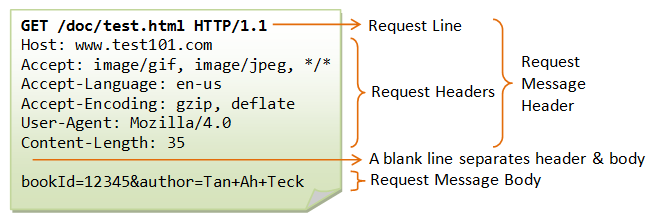
\includegraphics{HTTP_request_structure}
\caption{Cấu trúc một tập tin HTTP request cơ bản.}
\label{fig:http_req_struct}
\end{figure}

Cụ thể các đặc trưng được chọn để chuyển đổi thành vector như sau:

\begin{itemize}
\item \textbf{Length of the request} - Độ dài của request, cụ thể là đường dẫn của request bao gồm \emph{giao thức, domain, đường dẫn của file, các query (tham số)}.
\item \textbf{Length  of the arguments} - Độ dài của các tham số.
\item \textbf{Number of arguments} - Số lượng tham số
\item \textbf{Number of digits in the arguments} - Số lượng chữ số trong các tham số.
\item \textbf{Length of the path} - Độ dài của đường dẫn rút gọn, bao gồm \emph{giao thức, domain, đường dẫn của file}
\item \textbf{Number of `special' chars in request} - Số lượng kí tự nhận dạng mẫu đặc biệt xuất hiện trong request bao gồm \{\emph{script, select, from, where, update, drop, table, delete, or, and, alert}\}
\end{itemize}

Để hiểu rõ hơn các đặc trưng được chọn, xem xét một vài HTTP request được rút ra từ tập CISC 2010.

\begin{example}
Một HTTP request từ trong tập \emph{normal} (bình thường) như sau:

\begin{lstlisting}
GET http://localhost:8080/tienda1/publico/anadir.jsp?id=3&nombre=Vino+Rioja&precio=100&cantidad=55&B1=A%F1adir+al+carrito HTTP/1.1
User-Agent: Mozilla/5.0 (compatible; Konqueror/3.5; Linux) KHTML/3.5.8 (like Gecko)
Pragma: no-cache
Cache-control: no-cache
Accept: text/xml,application/xml,application/xhtml+xml,text/html;q=0.9,text/plain;q=0.8,image/png,*/*;q=0.5
Accept-Encoding: x-gzip, x-deflate, gzip, deflate
Accept-Charset: utf-8, utf-8;q=0.5, *;q=0.5
Accept-Language: en
Host: localhost:8080
Cookie: JSESSIONID=81761ACA043B0E6014CA42A4BCD06AB5
Connection: close
\end{lstlisting}
\end{example} 

Tiến hành phân tích các đặc trưng được chọn trong ví dụ trên:

\begin{itemize}
\item Length of the request: \lstinline{http://localhost:8080/tienda1/publico/anadir.jsp?id=3&nombre= Vino+Rioja&precio=100&cantidad=55&B1=A%F1adir+al+carritop}{} $\to$ \textbf{117}
\item Length of the arguments: \lstinline{id=3&nombre=Vino+Rioja&precio=100&cantidad=55&B1=A%F1adir+al+carrito}{} $\to$ \textbf{68}
\item Number of arguments: \textbf{5}
\item Number of digits in the arguments: \{\emph{3, 1, 0, 0, 5, 5, 1}\} $\to$ \textbf{7}
\item Length of the path: \lstinline{http://localhost:8080/tienda1/publico/anadir.jsp} $\to$ \textbf{39}
\item Number of `special' chars in request: \textbf{0}
\end{itemize}

Từ đó có được vector đầu vào với các giá trị \textbf{\{117, 68, 5, 7,48, 0\}} và có nhãn là \textbf{0} (tương ứng với traffic bình thường).

Xem xét thêm một ví dụ về một traffic bất thường.

\begin{example}
Một HTTP request từ trong tập \emph{anomalous} (bất thường) như sau:

\begin{lstlisting}
POST http://localhost:8080/tienda1/publico/anadir.jsp HTTP/1.1
User-Agent: Mozilla/5.0 (compatible; Konqueror/3.5; Linux) KHTML/3.5.8 (like Gecko)
Pragma: no-cache
Cache-control: no-cache
Accept: text/xml,application/xml,application/xhtml+xml,text/html;q=0.9,text/plain;q=0.8,image/png,*/*;q=0.5
Accept-Encoding: x-gzip, x-deflate, gzip, deflate
Accept-Charset: utf-8, utf-8;q=0.5, *;q=0.5
Accept-Language: en
Host: localhost:8080
Cookie: JSESSIONID=AE29AEEBDE479D5E1A18B4108C8E3CE0
Content-Type: application/x-www-form-urlencoded
Connection: close
Content-Length: 146

id=2&nombre=Jam%F3n+Ib%E9rico&precio=85&cantidad=%27%3B+DROP+TABLE+usuarios%3B+SELECT+*+FROM+datos+WHERE+nombre+LIKE+%27%25&B1=A%F1adir+al+carrito
\end{lstlisting}
\end{example} 

Tiến hành phân tích các đặc trưng được chọn trong ví dụ trên:

\begin{itemize}
\item Length of the request: \lstinline{http://localhost:8080/tienda1/publico/anadir.jsp}{} $\to$ \textbf{49}
\item Length of the arguments: \lstinline{id=2&nombre=Jam%F3n+Ib%E9rico&precio=85&cantidad=%27%3B+DROP+TABLE+usuarios%3B+SELECT+*+FROM+datos+WHERE+nombre+LIKE+%27%25&B1=A%F1adir+al+carrito}{}\\ $\to$ \textbf{146}
\item Number of arguments: \textbf{5}
\item Number of digits in the arguments: \{\emph{2, 3, 9, 8, 5, 2, 7, 3, 3, 2, 7, 2, 5, 1, 1}\} $\to$ \textbf{15}
\item Length of the path: \lstinline{http://localhost:8080/tienda1/publico/anadir.jsp} $\to$ \textbf{49}
\item Number of `special' chars in request: \textbf{\{DROP, TABLE, SELECT, FROM, WHERE, LIKE\}} $\to$ \textbf{6}
\end{itemize}

Từ đó có được vector đầu vào với các giá trị \textbf{\{49, 146, 5, 15, 49, 6\}} và có nhãn là \textbf{1} (tương ứng với traffic bất thường).

\subsubsection*{Hiện thực bằng Python}
Việc xử lí dữ liệu như trên sẽ được thực hiện thông qua đoạn code Python sau:

\begin{lstlisting}[language=Python]
# Global vars
file1 = "normalTrafficTraining.txt"
file2 = "anomalousTrafficTest.txt"

# Read normal traffic data
objfileNormal = read_file(file1)
# Process normal data
MatrixData, NumberRow = processFile(objfileNormal, 0)

# Read anomalous traffic data
objfileAnormal = read_file(file2)
#Process
MatrixAnomalous, NumberAnomalous = processFile(objfileAnormal, 1)

# Merge normal and anomalous data into one
MatrixData = np.vstack([MatrixData, MatrixAnomalous])

# Update number row of matrix
NumberRow = NumberRow + NumberAnomalous

# Save data
SaveModel(MatrixData, "MatrixData.pkl")
\end{lstlisting}

Hàm \textbf{read\_file} sẽ đọc lần lược file ``normalTrafficTraining.txt''  là tập dữ liệu gồm những request bình thường và  ``anomalousTrafficTest.txt'' là tập dữ liệu gồm những request bất thường. Hàm \textbf{processFile} trả về một ma trận, các dòng trong ma trận là các điểm dữ liệu được trích xuất từ HTTP request và số dòng của ma trận. Ma trận này gồm 7 cột, 6 cột đầu tương ứng với các đặc tính được trình bày ở trên. Cột thứ 7 là nhãn của dữ liệu gồm 0 hoặc 1 tương ứng bình thường hay bất thường.

\subsection{Phân tách dữ liệu huấn luyện và dữ liệu kiểm tra}
Tiến hành chia dữ liệu thành hai phần. Phần 1 gồm dữ liệu dùng để huấn luyện, chiếm 80\% dữ liệu. Phần 2 gồm dữ liệu cho quá trình kiểm tra độ chính xác chiếm 20\% dữ liệu.

Đoạn code Python sau được dùng để phân tách dữ liệu ra 2 phần:

\begin{lstlisting}[language=Python]
# Shuffle data
np.random.shuffle(MatrixData)

# Number of row for trainning data (80%)
NumberRowTrainSet = int(0.8 * NumberRow)

X_Train = MatrixData[0 : NumberRowTrainSet, 0 : NumberFeature]
Y_Train = MatrixData[0 : NumberRowTrainSet, NumberFeature]
X_Test = MatrixData[NumberRowTrainSet : NumberRow, 0 : NumberFeature]
Y_Test = MatrixData[NumberRowTrainSet : NumberRow, NumberFeature]
\end{lstlisting}

Để đảm bảo dữ liệu phân bố trộn lẫn các nhãn đều, trước khi tách ta tiến hành trộn dữ liệu. Sau khi trộn, tạo ra được 4 biến:

\begin{itemize}
\item \textbf{X\_Train} là tập gồm các giá trị đặc tính cho quá trình huấn luyện.
\item \textbf{Y\_Train} là tập gồm các nhãn của dữ liệu dùng cho quá trình huấn luyện.
\item Tương tự \textbf{X\_Test} và \textbf{Y\_Test} được dùng cho quá trình kiểm tra.
\end{itemize}

\subsection{Giai đoạn huấn luyện và kiểm tra}
Trong code minh họa dưới đây sử dụng thư viện của scikit-learn để hỗ trợ quá trình xây dựng cây. Cách thuật toán hoạt động đã được trình bày ở phần lý thuyết ở trên.

\begin{lstlisting}[language=Python]
# Training process
clf = tree.DecisionTreeClassifier(criterion="gini")
clf = clf.fit(X_Train, Y_Train)

# Save model to reuse
SaveModel(clf, "ModelDecisionTree.pkl")

# Show depth of tree
print("Depth of tree is: " + str(clf.tree_.max_depth))
\end{lstlisting}

Trong code có bước lưu lại mô hình cây thu được sau quá trình huấn luyện, có thể sử dụng lại mà không cần xây dựng lại từ đầu.

Sau khi tạo thành công cây, sử dụng tập \textbf{X\_Test} để dự đoán:

\begin{lstlisting}[language=Python]
# Predict
result = clf.predict(X_Test)
accuracy = accuracy_score(Y_Test, result)
print("Accuracy is: " + str(accuracy))

# Show report of predict
print(classification_report(Y_Test, result))
\end{lstlisting}

Biến \textbf{result} lưu giá trị dự đoán cho mỗi điểm dữ liệu trong \textbf{X\_Test}.

Dùng hàm \textbf{accuracy\_score()} để tính độ chính xác của kết quả dự đoán so với thực tế.

Hàm \textbf{classification\_report()} dùng để xuất báo cáo về thông số kết quả dự đoán. 

Report tổng quan mà phần mềm xuất ra được thể hiện như trong hình \ref{fig:result}.

\begin{figure}[ht!]
\centering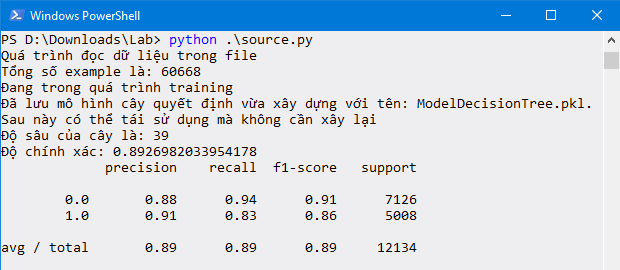
\includegraphics[scale=0.8]{result}
\caption{Kết quả từ chương trình khi chạy}
\label{fig:result}
\end{figure}

Tổng cộng \textbf{60668} dữ liệu thu được từ hai tập dữ liệu. Sau quá trình huấn luyện, kết quả dự đoán chính xác \textbf{0.8927} tức 89.27\%.

Giải thích thông số trong phần report:

\begin{itemize}
\item \textbf{Precision} là tỉ lệ dự đoán bất thường chính xác trong số tất cả các dự đoán bất thường (dù đúng hay sai).

\begin{displaymath}
\text{Precision} = \frac{\text{TP}}{\text{TP} + \text{FP}} 
\end{displaymath}

Trong đó:

\begin{itemize}
\item \textbf{TP} là số dự đoán điểm dữ liệu là bất thường chính xác.
\item \textbf{FP} là số dự đoán điểm dữ liệu là bất thường nhưng sai.
\end{itemize}

\item \textbf{Recall} là tỉ lệ dự đoán bất thường chính xác so với thực tế.

\begin{displaymath}
\text{Recall} = \frac{\text{TP}}{\text{TP} + \text{FN}}
\end{displaymath}

Trong đó, \textbf{FN} là số dự đoán điểm dữ liệu là bình thường nhưng sai.

\item \textbf{F1-score} là cân bằng giá trị giữa \emph{Precision} và \emph{Recall}. 

\begin{displaymath}
\text{F1-score} = 2\frac{\text{Precision}\cdot \text{Recall}}{\text{Precision} + \text{Recall}}
\end{displaymath}

chỉ cần quan tâm tới \textbf{F1-score}, giá trị càng cao càng tốt.
\item Cột support hiện số lượng dữ liệu của từng nhãn tương ứng.
\item Dòng cuối cùng là giá  trị trung bình và tổng cộng số lượng các nhãn.
\end{itemize}

Tiếp theo sẽ vẽ đồ thị \textbf{curves}, đồ thị curves thể hiện giá trị dự đoán chính xác trên tập dữ liệu huấn luyện (\emph{Training Set}) và tập dữ liệu điều chỉnh tham số (\emph{Cross Validation}). Trục tung là mức độ chính xác, \textbf{0} tức dự đoán sai hoàn toàn, \textbf{1} tức dự đoán đúng hoàn toàn. Trục hoành chỉ số lượng dữ liệu được đưa vào tính toán.

Giá trị được tính bằng cách ứng với một lượng dữ liệu nào đó, sẽ dùng để tạo cây quyết định. Sau đó dùng cây này để dự đoán lại trên tập dữ liệu mới được dùng để tạo cây, thu được giá trị độ chính xác, gọi nó là \textbf{Training score} và tiếp tục dùng cây này để dự đoán trên tập dữ liệu \textbf{Cross-Validation} thu được giá trị độ chính xác, gọi nó là \textbf{Cross-Validation Score}. Từ đó vẽ lên đồ thị như hình \ref{fig:res_curves}.

\begin{figure}[ht!]
\centering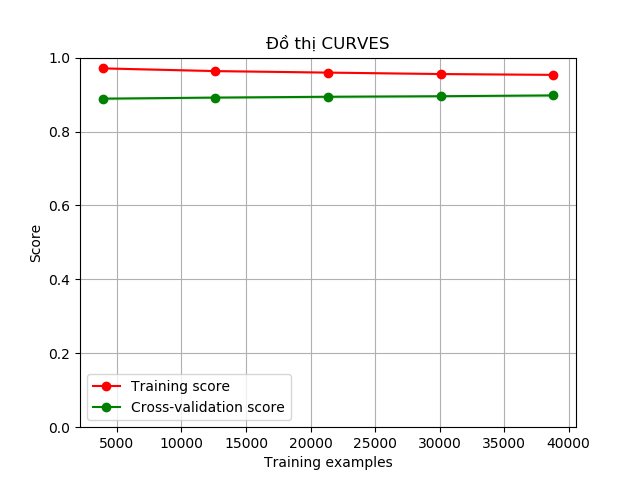
\includegraphics[scale=0.9]{curves}
\caption{Đồ thị curves thể hiện giá trị dự đoán chính xác}
\label{fig:res_curves}
\end{figure}

Sau khi quan sát đồ thị thấy đường màu đỏ (\emph{Training Score}) và đường màu xanh (\emph{Cross-Validation Score}) có xu hướng chạm nhau khi dữ liệu tăng lên. Hay nói cách khác, tuy độ chính xác trên tập huấn luyện càng giảm nhưng độ chính xác trên tập kiểm thử lại tăng. Đây là dấu hiệu tốt, chứng tỏ không bị vấn đề overfitting hoặc underfitting.

Để thêm trực quan, chúng tôi cũng cho xuất một file output là \textbf{DACN.pdf} cùng thư mục với file chạy thể hiện sơ đồ cây thu được.
\subsection{Điều chỉnh thông số}
Như đã trình bày ở phần \ref{sec:stop_trees}, để tăng độ chính xác và giảm thiểu trường hợp \emph{overfitting} có thể giới hạn độ sâu, số lượng điểm dữ liệu tối thiểu được phép tách node thành hai nhánh mới hoặc số điểm dữ liệu tối thiểu phải có trên một nút lá và nhiều thông số khác. Tiến hành thử từng thông số, mỗi thông số sau quá trình huấn luyện sẽ được kiểm thử và tính chỉ số \textbf{F1-score}. Cuối cùng chọn bộ tham số có chỉ số F1-score cao nhất.

Quá trình chọn tham số được giải quyết qua thư viện \textbf{GridSearchCV} trong scikit-learn. Thư viện sẽ tiến hành thử từng bộ tham số, cho ta kết quả tốt nhất.

\begin{lstlisting}[language=Python]
paramater = [{'max_depth' : range(1, 40), 'min_samples_split' : range(2,50), 'min_samples_leaf' : range(1,10)}]
clf = GridSearchCV(tree.DecisionTreeClassifier(), paramater, cv=10,n_jobs=6)
clf = clf.fit(X_Train, Y_Train)
\end{lstlisting}

Biến \textbf{paramater} liệt kê những tham số cần thay đổi, trong báo cáo này ba thông số sau sẽ được thay đổi:

\begin{itemize}
\item \textbf{max\_depth:} độ sâu tối đa của cây, lần lượt thử từ $1 \to 40$.
\item \textbf{min\_samples\_split:} số lượng điểm dữ liệu tối thiểu cho phép tách, $2 \to 50$.
\item \textbf{min\_samples\_leaf:} số lượng điểm dữ liệu tối thiểu phải có ở node lá, $1 \to 10$.
\end{itemize}

Trong quá trình điều chỉnh tham số, sử dụng \textbf{cv=10}, cv tức \emph{cross-validation}, phần dữ liệu để tính toán F1-score ứng với mỗi bộ tham số. Giá trị \textbf{10} ở đây tức chia tập dữ liệu thành 10 phần, ta chỉ dùng 9 phần để để train, phần thứ 10 để tính độ hiểu quả của cây (F1-score).

Kết quả sau khi điều chỉnh tham số được xuất ra như ở hình \ref{fig:result_2}.

\begin{figure}[ht!]
\centering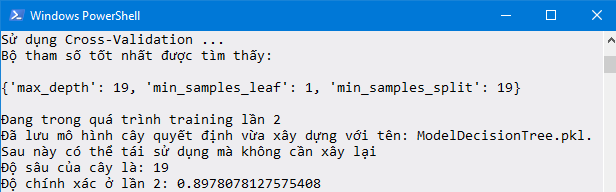
\includegraphics[scale=0.9]{result_2}
\caption{Kết quả sau khi điều chỉnh tham số}
\label{fig:result_2}
\end{figure}

Ứng với bộ tham số tốt nhất tìm được là: \textbf{max\_depth} = 19; \textbf{min\_samples\_leaf} = 1; \textbf{min\_samples\_split} = 19  thấy có trung bình độ chính xác cao nhất \textbf{0.901} độ lệch chuẩn \textbf{0.008}. Sau khi dùng bộ tham số này độ chính xác của thuật toán được cải thiện từ $0.8927$ đến $0.8978$.

Ở phần này cũng thực hiện cập nhật lại mô hình cây vào tập tin \textbf{ModelDecisionTree.pkl} để thuận tiện cho việc dùng lại mô hình.

\section{Kết luận và hướng phát triển}
Báo cáo này đã chỉ ra một phương pháp mới, tiên tiến hơn để phát hiện tấn công ứng dụng web. Đó là áp dụng \gls{ml} để giải quyết bài toán với thuật toán cây quyết định, họ CART. Kết quả quan sát được rất tốt, dựa vào tập dữ liệu CSIC 2010 với xác suất dự đoán kiểm thử đạt gần 90\%.

Nhược điểm là những đặc tính được chọn để hình thành vector chưa khai khác hết những gì tập dữ liệu CSIC mang lại. Do chưa có kiến thức đủ vững về giao thức HTTP cũng như các loại tấn công nên những trường dữ liệu như: user-agent, pragma, cache, accept, cookie, \ldots chưa được khai thác triệt để. Còn nhiều loại thuật toán phân loại khác như: \emph{Naive Bayes, Logistic Regression, Support Vector Machne, Random Forest}, \ldots là những thuật toán cơ bản, nổi tiếng không kém cây quyết định. Nhưng vì thời gian có hạn nên chưa thể triển khai trên các thuật toán này.

Hướng phát triển:

\begin{itemize}
\item Tìm hiểu sâu hơn về giao thức HTTP để hiểu và vận dụng tốt các trường để khai thác tối đa đặc tính tạo thành vector.
\item Tìm hiểu nhiều hơn về các giao thức tấn công web để cải tiến mô hình phân loại nhận diện tấn công.
\item Triển khai trên các thuật toán phân loại khác, so sánh số liệu và rút ra kết luận. Tìm thuật toán tối ưu nhất trong những trường hợp nhất định.
\end{itemize}

\end{document}